\documentclass[%
    12pt,
    bibliography=toc,
    listof=leveldown,% use section for the list headings
    oneside
]{book}
\usepackage[subpreambles=true]{standalone}

\usepackage[margin=2cm]{geometry}
\usepackage[table]{xcolor}
\usepackage[utf8]{inputenc}
\usepackage[english]{babel}
\usepackage{listings}
\usepackage[toc,page]{appendix}
\usepackage{tikz}
\usepackage[absolute,overlay]{textpos}
\usepackage{etoolbox}
\usepackage{pdfpages}
\usepackage{tabularx}
\usepackage{hyperref}
\usepackage{import}
\usepackage{amsmath}
\usepackage{cleveref}

% Chapter formatting
\usepackage{titlesec, blindtext, color}
\definecolor{gray75}{gray}{0.75}
\newcommand{\hsp}{\hspace{20pt}}
\titleformat{\chapter}[hang]{\Huge\bfseries}{\thechapter\hsp\textcolor{gray75}{\textbar}\hsp}{0pt}{\Huge\bfseries}
\titlespacing*{\chapter}{0pt}{-40pt}{30pt}

\usepackage{stmaryrd}
\usepackage{framed}

\renewcommand{\leadsto}{\rightsquigarrow}
\providecommand{\dmid}{\ \parallel \ }

\providecommand{\effFalse}{\mathbf{false}}
\providecommand{\effTrue}{\mathbf{true}}
\providecommand{\effLeft}{\mathbf{Left}\ }
\providecommand{\effRight}{\mathbf{Right\ }}
\providecommand{\effFun}{\mathbf{fun}\ }
\providecommand{\effRecFun}{\mathbf{recfun}\ }
\providecommand{\effHandler}{\mathbf{handler}\ }
\providecommand{\effVal}{\mathbf{val}\ }
\providecommand{\effWith}{\mathbf{with}\ }
\providecommand{\effHandle}{\ \mathbf{handle}\ }
\providecommand{\effIf}{\mathbf{if}\ }
\providecommand{\effThen}{\ \mathbf{then}\ }
\providecommand{\effElse}{\ \mathbf{else}\ }
\providecommand{\effAbsurd}{\mathbf{absurd}\ }
\providecommand{\effMatch}{\mathbf{match}\ }
\providecommand{\effLet}{\mathbf{let}\ }
\providecommand{\effIn}{\ \mathbf{in}\ }
\providecommand{\effRec}{\mathbf{rec}\ }
\providecommand{\effEffect}{\mathbf{effect}\ }
\providecommand{\effFinally}{\mathbf{finally}\ }
\providecommand{\effOp}{\mathtt{op}}
\providecommand{\effPerform}{\mathbf{perform}\ }
\providecommand{\tto}{\twoheadrightarrow}

\providecommand{\handlerType}{\Rightarrow}
\providecommand{\boolType}{\mathtt{bool}}
\providecommand{\unitType}{\mathtt{unit}}
\providecommand{\emptyType}{\mathtt{empty}}

\providecommand{\defEq}{\stackrel{\text{def}}{=}}

\providecommand{\cek}[1]{\langle #1 \rangle}
\providecommand{\secd}[1]{\langle #1 \rangle}
\providecommand{\shade}[1]{\langle #1 \rangle}

\providecommand{\irId}{\mathbf{Id}}
\providecommand{\irConst}{\mathbf{Const}}
\providecommand{\irBox}{\mathbf{Box}}
\providecommand{\irFun}{\mathbf{Fun}}
\providecommand{\irHandler}{\mathbf{Handler}}
\providecommand{\irVal}{\mathbf{Return}}
\providecommand{\irIf}{\mathbf{If}}
\providecommand{\irLetIn}{\mathbf{LetIn}}
\providecommand{\irLetRecIn}{\mathbf{LetRecIn}}
\providecommand{\irTopLet}{\mathbf{TopLet}}
\providecommand{\irTopLetRec}{\mathbf{TopLetRec}}
\providecommand{\irPerform}{\mathbf{Perform}}
\providecommand{\irWithHandle}{\mathbf{WithHandle}}
\providecommand{\irBinOp}{\mathbf{BinOp}}
\providecommand{\irFunApp}{\mathbf{FunApp}}
\providecommand{\irGetField}{\mathbf{GetField}}
\providecommand{\irListHead}{\mathbf{ListHead}}
\providecommand{\irListTail}{\mathbf{ListTail}}

\providecommand{\interp}[1]{\llbracket #1 \rrbracket}

\providecommand{\shUnit}{\mathbf{()}}
\providecommand{\shHalt}{\mathbf{halt}}
\providecommand{\shCast}{\mathbf{cast}}
\providecommand{\shRett}{\mathbf{ret2}}
\providecommand{\shApply}{\mathbf{apply}}
\providecommand{\shCastShadow}{\mathbf{castshadow}}
\providecommand{\shKillShadow}{\mathbf{killshadow}}
\providecommand{\shFin}{\mathbf{fin}}
\providecommand{\shThrow}{\mathbf{throw}}

\providecommand{\vmPush}{\textbf{push}}
\providecommand{\vmPop}{\textbf{pop}}
\providecommand{\vmAcc}[1]{\textbf{acc} #1}
\providecommand{\vmConst}[1]{\textbf{const} #1}
\providecommand{\vmHalt}{\textbf{halt}}
\providecommand{\vmJump}[1]{\textbf{jump }#1}
\providecommand{\vmLabel}{\textbf{label}}
\providecommand{\vmBranchIfNot}[1]{\textbf{branchifnot }#1}
\providecommand{\vmApply}{\textbf{apply}}
\providecommand{\vmRet}{\textbf{ret}}
\providecommand{\vmRett}{\textbf{ret2}}
\providecommand{\vmMakeBox}[2]{\textbf{makebox }#1, #2}
\providecommand{\vmGetField}[1]{\textbf{getfield }#1}
\providecommand{\vmListHead}{\textbf{listhead}}
\providecommand{\vmListTail}{\textbf{listtail}}
\providecommand{\vmMakeClosure}[2]{\textbf{makeclosure }#1, #2}
\providecommand{\vmMakeHlosure}[4]{\textbf{makehlosure }#1, #2, #3, #4}
\providecommand{\vmThrow}{\textbf{throw}}
\providecommand{\vmFin}{\textbf{fin}}
\providecommand{\vmCastShadow}{\textbf{castshadow}}
\providecommand{\vmKillShadow}{\textbf{killshadow}}

\providecommand{\hlosure}{\mathcal{H}}
\providecommand{\konts}{\mathcal{C}}

\newenvironment{myfigure}[4][0.75]{
    \def\mywidth{#1}
    \def\mycaption{#3}
    \def\mylabel{#4}
    \definecolor{shadecolor}{rgb}{0.95,0.95,0.95}

    \begin{figure}[#2]
    \centering
    \begin{minipage}{\mywidth\textwidth}
    \begin{shaded*}
}{
    \caption{\mycaption}
    \label{\mylabel}
    \end{shaded*}
    \end{minipage}
    \end{figure}
}
\usepackage{color}
\usepackage{xcolor}
\usepackage{caption}
\usepackage{courier}

\lstdefinelanguage{efflang}
{
    % list of keywords
    morekeywords={
        let,
        perform,
        continue,
        val,
        effect,
        in,
        if, then, else,
        with, handle, handler,
        finally,
        match,
        exception,
        of
    },
    sensitive=false,
    morecomment=[s]{(*}{*)},
    morestring=[b]"
}

\lstdefinelanguage{scheme}
{
    % list of keywords
    morekeywords={
        define, call/cc, lambda
    },
    sensitive=false,
    morecomment=[s]{\#|}{|\#},
    morestring=[b]"
}

\lstset{
  basicstyle=\small\ttfamily, % Default font
  numberstyle=\small,          % Style of line numbers
  numbersep=5pt,              % Margin between line numbers and text
  tabsize=2,                  % Size of tabs
  extendedchars=true,
  breaklines=true,            % Lines will be wrapped
  keywordstyle=\color{red},
  frame=b,
  numbers=left,
  numberstyle=\footnotesize\color{gray},
  numbersep=10pt,
  captionpos=t,
  stringstyle=\color{purple!80!blue}\ttfamily, % Color of strings
  showspaces=false,
  showtabs=false,
  xleftmargin=17pt,
  framexleftmargin=17pt,
  framexbottommargin=4pt,
  showstringspaces=false
}

\DeclareCaptionFont{white}{\color{white}}
\DeclareCaptionFormat{listing}{\colorbox[cmyk]{0.43, 0.35, 0.35,0.01}{\parbox{\textwidth}{\hspace{15pt}#1#2#3}}}
\captionsetup[lstlisting]{format=listing,labelfont=white,textfont=white, singlelinecheck=false, margin=0pt, font={bf,footnotesize}}

\newcommand{\mylisting}[4]{%
\noindent
\begin{minipage}{\textwidth}
\lstinputlisting[
  language=#1,
  caption={#2},
  label=#3
  ]{#4}
\end{minipage}
  }

\lstset{language=efflang}

\begin{document}
\input titlepage

\frontmatter

\section*{Declaration of Originality}

I, Géza Csenger of Homerton College, being a candidate for Part II of the 
Computer Science Tripos, hereby declare that this dissertation and the work
described in it are my own work, unaided except as may be specified below, and
that the dissertation does not contain material that has already been used to
any substantial extent for a comparable purpose.

I, Géza Csenger of Homerton College,
am content for my dissertation to be made available to the students and staff
of the University. 

\vspace{1cm}
\textbf{Signed}

\vspace{1cm}
\textbf{Date}

\vspace{3cm}

\section*{Acknowledgements}

Hereby, I would like to say thanks to:
\begin{itemize}
    \item My project supervisor, \textbf{Prof.\ Alan Mycroft}, for his support
        and guidance
    \item My Director of Studies, \textbf{Dr John Fawcett}, for a \emph{lot} of
        things
    %\item Special thanks goes to Lili Janzer for proofreading this work as an \emph{actual} Part IB student
    \item Friends and family without whom completing this work would have been impossible
\end{itemize}

\newpage

\chapter{Proforma}
\begin{tabularx}{\textwidth}{@{} ll @{}}
Candidate number & 2375C \\
Project title & Compiling algebraic effect handlers \\
Examination & Computer Science Tripos -- Part II, 2020 \\
Word Count & 10314 \\
Lines of Code & 6158
\footnote{Obtained with Visual Studio Code's \href{https://marketplace.visualstudio.com/items?itemName=uctakeoff.vscode-counter}{VS Code Counter} extension} \\
Page Count & 40 \\
Project Originator & The author \\
Supervisor & Professor Alan Mycroft \\
\end{tabularx}

\paragraph{Original aims of the Project}

The project had four core aims: to write an interpreter for Eff, to design a
byte code for Eff, to write a compiler from Eff to this byte code and to
implement a virtual machine interpreting the byte code. Additional goals were
to implement various optimisations for Eff, such as tail resumption optimisation
or minimising the copy overhead from the use of continuations.

\paragraph{Work completed}

A syntax-level Eff interpreter was implemented. A byte code for Eff (SHADEcode)
was designed. A compiler from Eff to SHADEcode was implemented as well as a
virtual machine (SHADE) interpreting SHADEcode. As far as I know, SHADE and
SHADEcode are the first virtual machine and byte code designed
\emph{specifically} for Eff. In the Evaluation chapter I compare the performance
of my Eff interpreter with the current official Eff interpreter and the
performance of the SHADE virtual machine with the performance of Multicore
OCaml (another compiled language with similar features to Eff).

\paragraph{Special difficulties}
None.

\tableofcontents

\newpage
\listoffigures
\listoftables
\lstlistoflistings

\mainmatter

\chapter{Introduction}
\import{sections/}{introduction}

\chapter{Preparation}
\import{sections/}{preparation}

\chapter{Implementation}
\import{sections/}{implementation}

\chapter{Evaluation}
\import{sections/}{evaluation}

\chapter{Conclusion}
\import{sections/}{conclusion}

\bibliography{bibliography}{}
\bibliographystyle{plain}

\appendix

\begin{appendices}
\renewcommand{\thepage}{\thechapter.\arabic{page}}

\chapter{Theory}
\label{app:theory}
\setcounter{page}{1}
\import{sections/}{theory}

\chapter{Code snippets}
\label{code-snippets}
\setcounter{page}{1}
\import{sections/}{code_snippets}

\chapter{Software Engineering}
\label{app:softeng}
\setcounter{page}{1}
\import{sections/}{softeng}

\chapter{Measurement results}
\label{raw-data}
\setcounter{page}{1}
\import{sections/}{measurement}

\chapter{Project Proposal}
\label{project-proposal}
\setcounter{page}{1}
The project proposal starts on the next page.
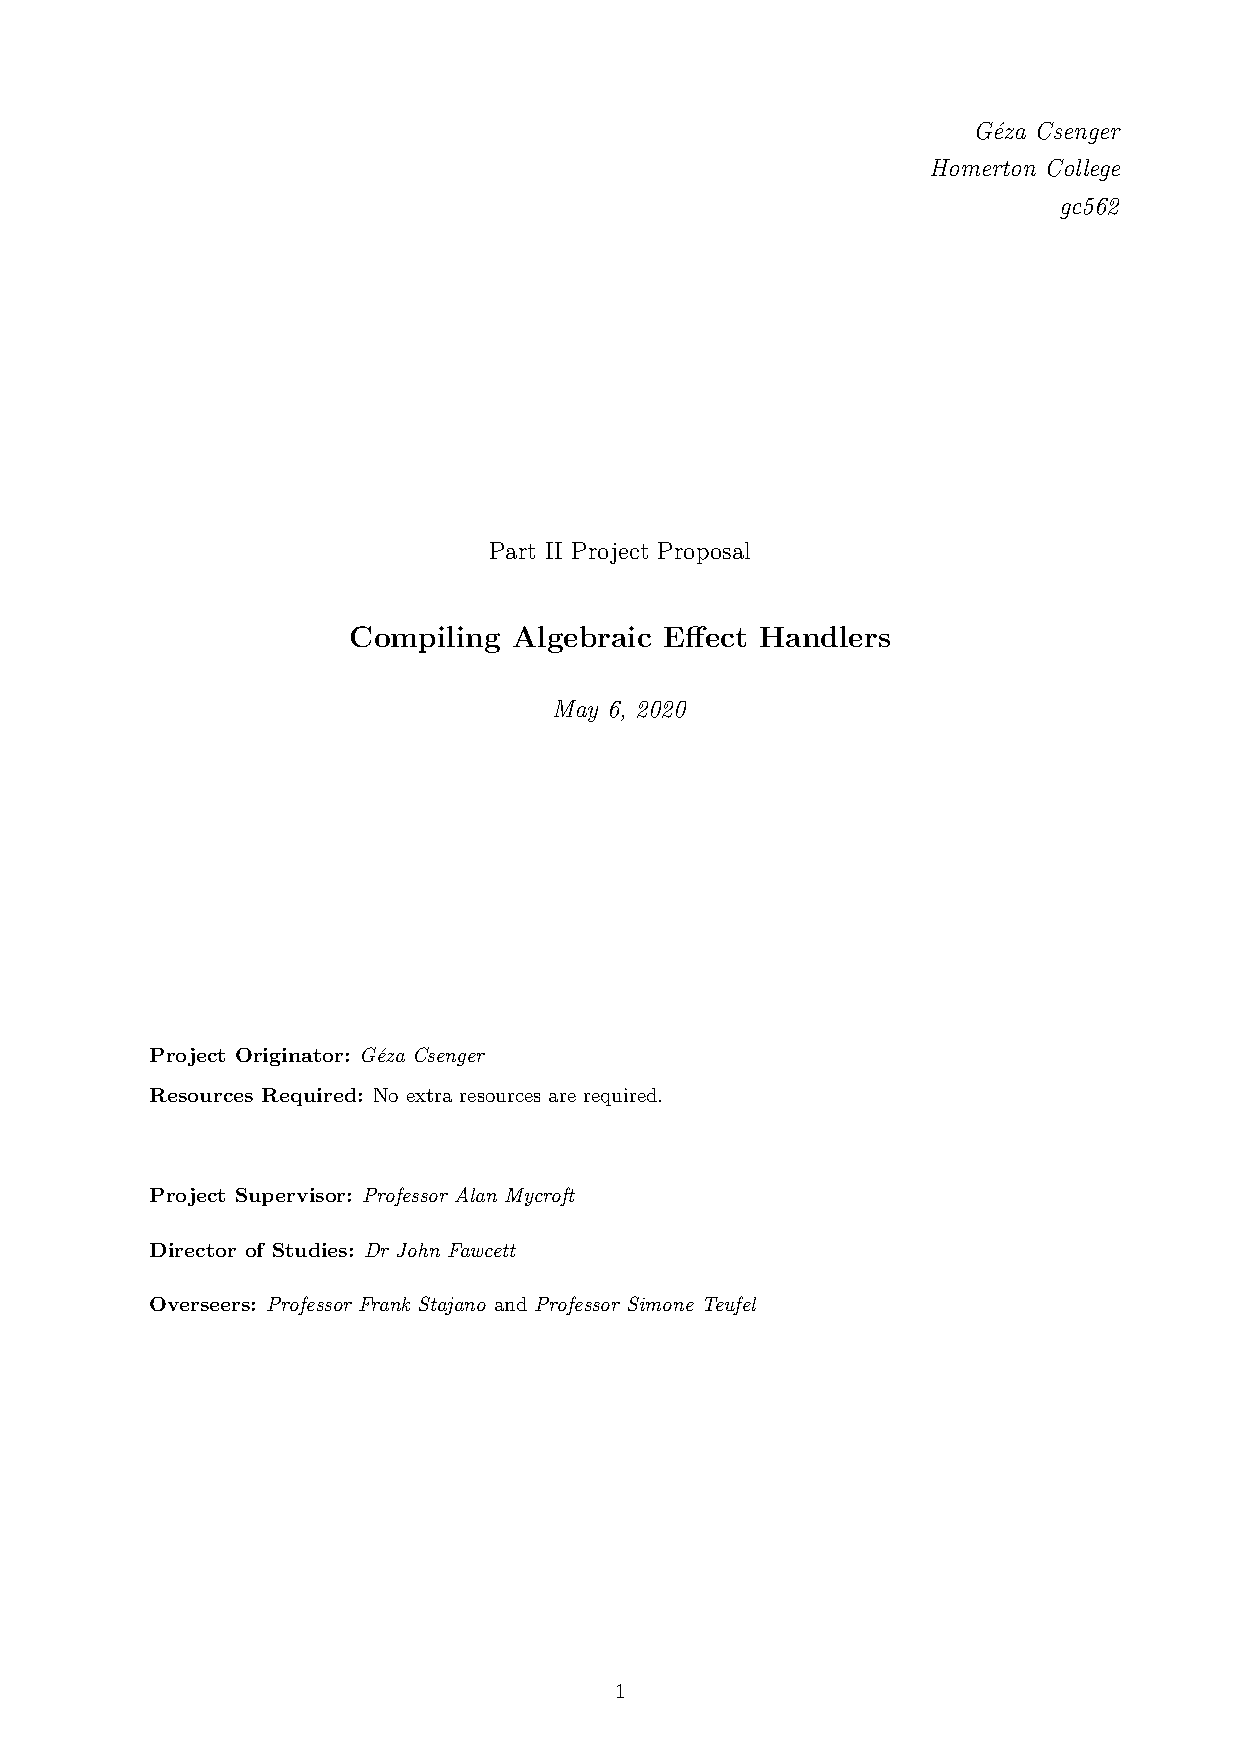
\includepdf[pages=-]{sections/proposal.pdf}

\end{appendices}

\end{document}
